\ylDisplay{Kondensaatorid} % Ülesande nimi
{Mihkel Rähn} % Autor
{piirkonnavoor} % Voor
{2006} % Aasta
{G 7} % Ülesande nr.
{6} % Raskustase
{
% Teema: Elektriahelad
\ifStatement
\begin{wrapfigure}{r}{0.45\textwidth}
	\begin{center}
		\vspace{-25pt}
		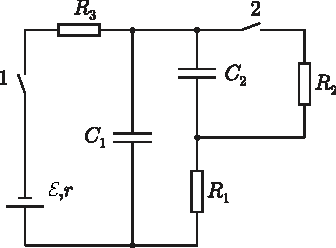
\includegraphics[width=\linewidth]{2006-v2g-07-yl}
	\end{center}
\end{wrapfigure}
Joonisel toodud elektriskeemil on vooluallikas elektromotoorjõuga $\mathcal E$ ja sisetakistusega $r$, kolm takistit takistustega $R_1 = R_2 = R_3 = R$ ning kondensaatorid mahtuvustega $C_1$ ja $C_2$. Arvutage, kui suured on elektrilaengud kondensaatoritel pärast pika aja möödumist, kui:\\
\osa lüliti 1 on suletud, lüliti 2 on avatud;\\
\osa mõlemad lülitid on suletud;\\
\osa eelmisest seisust avatakse mõlemad lülitid üheaegselt. 
\fi


\ifHint
\osa\osa Peale pikka aega on kondensaatoreid läbiv vool null, sest nende pinged, ja seega laengud, on stabiliseerunud. Seega võib kondensaatorid efektiivselt süsteemist välja lõigata.\\
\osa Elimineerides süsteemist vooluallika, peab kehtima laengu jäävuse seadus.
\fi


\ifSolution
\osa Vooluallikas laeb mõlemad kondensaatorid elektromotoorjõuga võrdse pingeni, seega on $q_{a1} = C_1\mathcal E$ ja $q_{a2} = C_2\mathcal E$.\\
\osa Leiame, kui suure pingeni kondensaatoreid laaduvad. Voolutugevus ahelas
on
\[
I = \frac{\mathcal E}{R_1+R_2+R_3+r}.
\]
Kondensaatoril $C_1$ on laeng $q_{b1} = C_1I(R_1 + R_2)$ ja kondensaatoril $C_2$ on laeng $q_{b2} = C_2IR_2$.\\
\osa Kehtib laengu jäävus, paralleelses ühenduses on pinged kondensaatoritel võrdsed. Summaarne laeng $q = q_{b1} + q_{b2}$ ning mahtuvus $C = C_1 + C_2$. Pinge kondensaatoril on $U = q/C$. Laengud kondensaatoritel on $q_{c1} = C_1U$ ja $q_{c2} = C_2U$. 
\fi
}